\documentclass[tikz,border=3pt]{standalone}
\usepackage{tikz-feynman}
\begin{document}
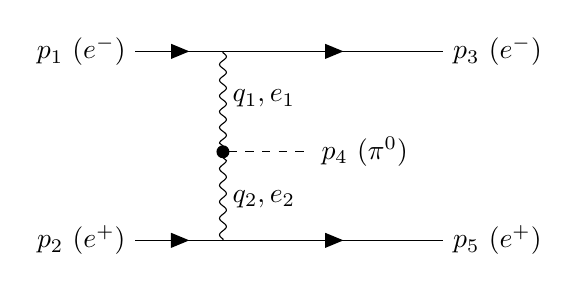
\begin{tikzpicture}
\begin{feynman}
\vertex (p1) {\(p_1\) (\(e^-\))};
\vertex[right=1.8cm of p1] (A);
\vertex[right=2.8cm of A] (p3) {\(p_3\) (\(e^-\))};
\vertex[below=2.4cm of p1] (p2) {\(p_2\) (\(e^+\))};
\vertex[right=1.8cm of p2] (B);
\vertex[right=2.8cm of B] (p5) {\(p_5\) (\(e^+\))};
\vertex[right=2.8cm of A, below=1.2cm of A, dot] (C) {};
\vertex[right=1.8cm of C] (p4) {\(p_4\) (\(\pi^0\))};

\diagram* {
  (p1) -- [fermion] (A) -- [fermion] (p3),
  (p2) -- [fermion] (B) -- [fermion] (p5),
  (A) -- [photon, edge label={\(q_1,e_1\)}] (C),
  (B) -- [photon, edge label'={\(q_2,e_2\)}] (C),
  (C) -- [scalar] (p4),
};
\end{feynman}
\end{tikzpicture}
\end{document}
